\documentclass[11pt]{beamer}
\usepackage[utf8]{inputenc}
\usepackage[T1]{fontenc}
\usepackage{amsmath}
\usepackage{amsfonts}
\usepackage{amssymb}
\usepackage{graphicx}
\usepackage{listings}
\usepackage{color}

\usetheme{default}

\definecolor{codegreen}{rgb}{0,0.6,0}
\definecolor{codegray}{rgb}{0.5,0.5,0.5}
\definecolor{codepurple}{rgb}{0.58,0,0.82}
\definecolor{backcolour}{rgb}{0.95,0.95,0.92}

\lstdefinestyle{mystyle}{
	backgroundcolor=\color{backcolour},   
	commentstyle=\color{codegreen},
	keywordstyle=\color{magenta},
	numberstyle=\tiny\color{codegray},
	stringstyle=\color{codepurple},
	basicstyle=\tiny,
	breakatwhitespace=false,         
	breaklines=true,                 
	captionpos=b,                    
	keepspaces=true,                 
	numbers=left,                    
	numbersep=5pt,                  
	showspaces=false,                
	showstringspaces=false,
	showtabs=false,                  
	tabsize=2
}

%\lstset{style=mystyle}

\lstdefinelanguage{JavaScript}{
	keywords={typeof, new, true, false, catch, function, return, null, catch, switch, var, if, in, while, do, else, case, break},
	keywordstyle=\color{blue}\bfseries,
	ndkeywords={class, export, boolean, throw, implements, import, this},
	ndkeywordstyle=\color{darkgray}\bfseries,
	identifierstyle=\color{black},
	sensitive=false,
	comment=[l]{//},
	morecomment=[s]{/*}{*/},
	commentstyle=\color{purple}\ttfamily,
	stringstyle=\color{red}\ttfamily,
	morestring=[b]',
	morestring=[b]"
}

\lstset{
	style=mystyle,
	language=JavaScript,
	backgroundcolor=\color{lightgray},
	extendedchars=true,
	basicstyle=\footnotesize\ttfamily,
	showstringspaces=false,
	showspaces=false,
	numbers=left,
	numberstyle=\footnotesize,
	numbersep=9pt,
	tabsize=2,
	breaklines=true,
	showtabs=false,
	captionpos=b
}

\begin{document}
	\author{Musa Baloyi}
	\title{Introduction to Chatbots \\ Introduction to IBM Watson} %Intermediate
	%\subtitle{}
	%\logo{}
	%\institute{}
	%\date{}
	%\subject{}
	%\setbeamercovered{transparent}
	%\setbeamertemplate{navigation symbols}{}
	\begin{frame}[plain]
	\maketitle
\end{frame}

\begin{frame}
	\frametitle{Introduction to IBM Watson}
	\begin{enumerate}
		\item Recap: State of the art
		\item Services
		%\item Data collection opt-out
		\item Programming languages
		\item Databases
		\item Programming environments
		\item Getting started tutorial (part one)
		\item References
	\end{enumerate}
\end{frame}

%\begin{frame}
%\frametitle{Recap: State of the art}
%	\begin{enumerate}
%	\item Basic Introduction
%	\begin{enumerate}
%		\item Motivation
%		\item Definitions
%		\item Types
%		\item Applications
%	\end{enumerate}
%	\item Technology Providers
%	\begin{enumerate}
%		\item Overview
%		%\item Slack
%		\item Telegram
%		%\item Facebook Messenger
%		\item IBM Watson
%	\end{enumerate}
%\end{enumerate}
%\end{frame}

\begin{frame}
	\frametitle{Services}
	\begin{enumerate}
		\item Authorization
		\item Assistant
		\item Discovery
		\item Language Translator
		\item Natural Language Classifier
		\item Natural Language Understanding
		\item Personality Insights
		\item Speech to Text
		\item Text to Speech
		\item Tone Analyzer
		\item Visual Recognition
	\end{enumerate}
\end{frame}

\begin{frame}
	\frametitle{Authorization}
	\begin{itemize}
		\item The Authorization service can generate auth tokens for situations where providing the service username/password is undesirable.
		\item Tokens are valid for 1 hour
		\item Services now use Identity and Access Management (IAM) authentication
		\item To access API methods by using IAM, you must first collect the credentials from the service dashboard.
		\item IBM recommends that you use authentication to generate the access token. 
		\begin{figure}[h]
			\centering
			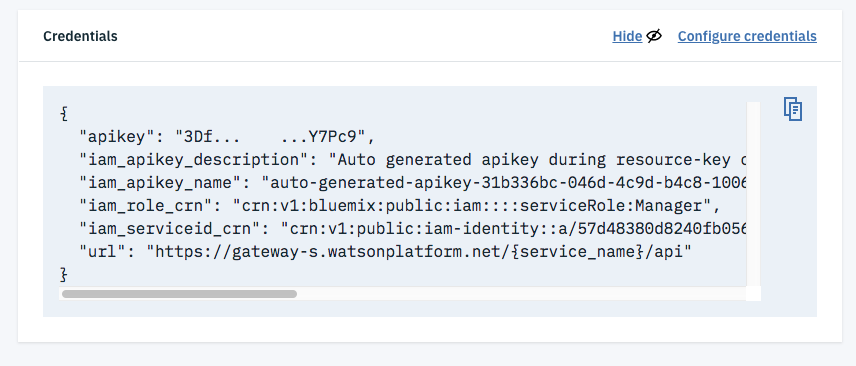
\includegraphics[scale=.2]{images/IAM-apikey}
			\label{IAM-apikey}
		\end{figure}
	
	%	\begin{figure}[h]
	%		\centering
	%		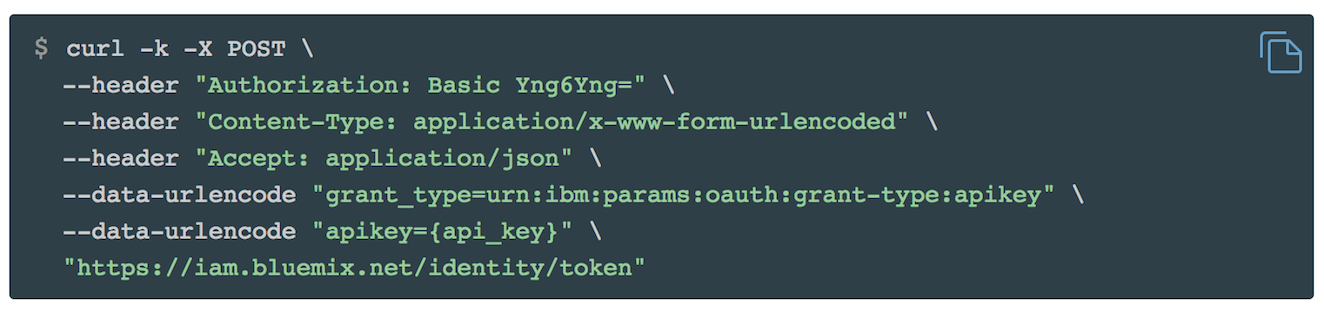
\includegraphics[scale=.2]{images/auth-curl-identity-token}
	%		\label{auth-curl-identity-token}
	%	\end{figure}
		
	\end{itemize}
\end{frame}

\begin{frame}
	\frametitle{Assistant}
	\begin{itemize}
		\item Formerly Conversation
		\item Use the Assistant service to determine the intent of a message.
	\end{itemize}
	\lstinputlisting[language=Javascript]{assistant1.js}
\end{frame}

\begin{frame}
	\frametitle{Discovery}
	\begin{itemize}
		\item Use the Discovery Service to search and analyze structured and unstructured data.
	\end{itemize}
	\lstinputlisting[language=Javascript]{discovery1.js}
\end{frame}

\begin{frame}
\frametitle{Language Translator}
	\begin{itemize}
		\item Translate text from one language to another or idenfity a language using the Language Translator service.
	\end{itemize}
	\lstinputlisting[language=Javascript]{translator1.js}
\end{frame}

\begin{frame}
	\frametitle{Natural Language Classifier}
	\begin{itemize}
		\item Use Natural Language Classifier service to create a classifier instance by providing a set of representative strings and a set of one or more correct classes for each as training. 
		\item Then use the trained classifier to classify your new question for best matching answers or to retrieve next actions for your application.
	\end{itemize}
	\lstinputlisting[language=Javascript]{nlclassifier1.js}
\end{frame}

\begin{frame}
	\frametitle{Natural Language Understanding}
	\begin{itemize}
		\item Use Natural Language Understanding is a collection of natural language processing APIs that help you understand sentiment, keywords, entities, high-level concepts and more.
		\item The fs module allows you to work with the file system on your computer.
	\end{itemize}
	\lstinputlisting[language=Javascript]{nlunderstanding1.js}
\end{frame}


\begin{frame}
	\frametitle{Personality Insights}
	\begin{itemize}
		\item Analyze text in English and get a personality profile by using the Personality Insights service.
	\end{itemize}
	\lstinputlisting[language=Javascript]{personality1.js}
\end{frame}

\begin{frame}
	\frametitle{Speech to Text}
	\begin{itemize}
		\item Use the Speech to Text service to recognize the text from a .wav file.
	\end{itemize}
	\lstinputlisting[language=Javascript]{speech_to_text1.js}
\end{frame}

\begin{frame}
	\frametitle{Text to Speech}
	\begin{itemize}
		\item Use the Text to Speech service to synthesize text into a .wav file.
	\end{itemize}
	\lstinputlisting[language=Javascript]{text_to_speech1.js}
\end{frame}

\begin{frame}
	\frametitle{Tone Analyzer}
	\begin{itemize}
		\item Use the Tone Analyzer service to analyze the emotion, writing and social tones of a text.
	\end{itemize}
	\lstinputlisting[language=Javascript]{tone_analyzer1.js}
\end{frame}

\begin{frame}
	\frametitle{Visual Recognition}
	\begin{itemize}
		\item Use the Visual Recognition service to recognize pictures.
	\end{itemize}
	\lstinputlisting[language=Javascript]{visual_recognition1.js}
\end{frame}


\begin{frame}
\frametitle{Development support}
\begin{itemize}
	\item NodeJS
	\item Python
	\item Java
	\item .Net
	\item Ruby
	\item Swift
	\item Unity
	\item Salesforce Apex
	\item Botkit
	\item Spring Boot
	\item Android
\end{itemize}
\end{frame}

\begin{frame}
\frametitle{Databases}
\begin{itemize}
	\item Cloudant
\end{itemize}
\end{frame}

\begin{frame}
\frametitle{Programming environments}
\begin{itemize}
	\item CloudFoundry
	\item IBM Cloud, formerly BlueMix
\end{itemize}
\end{frame}

\begin{frame}
\frametitle{Assistant}
\begin{figure}[h]
	\centering
	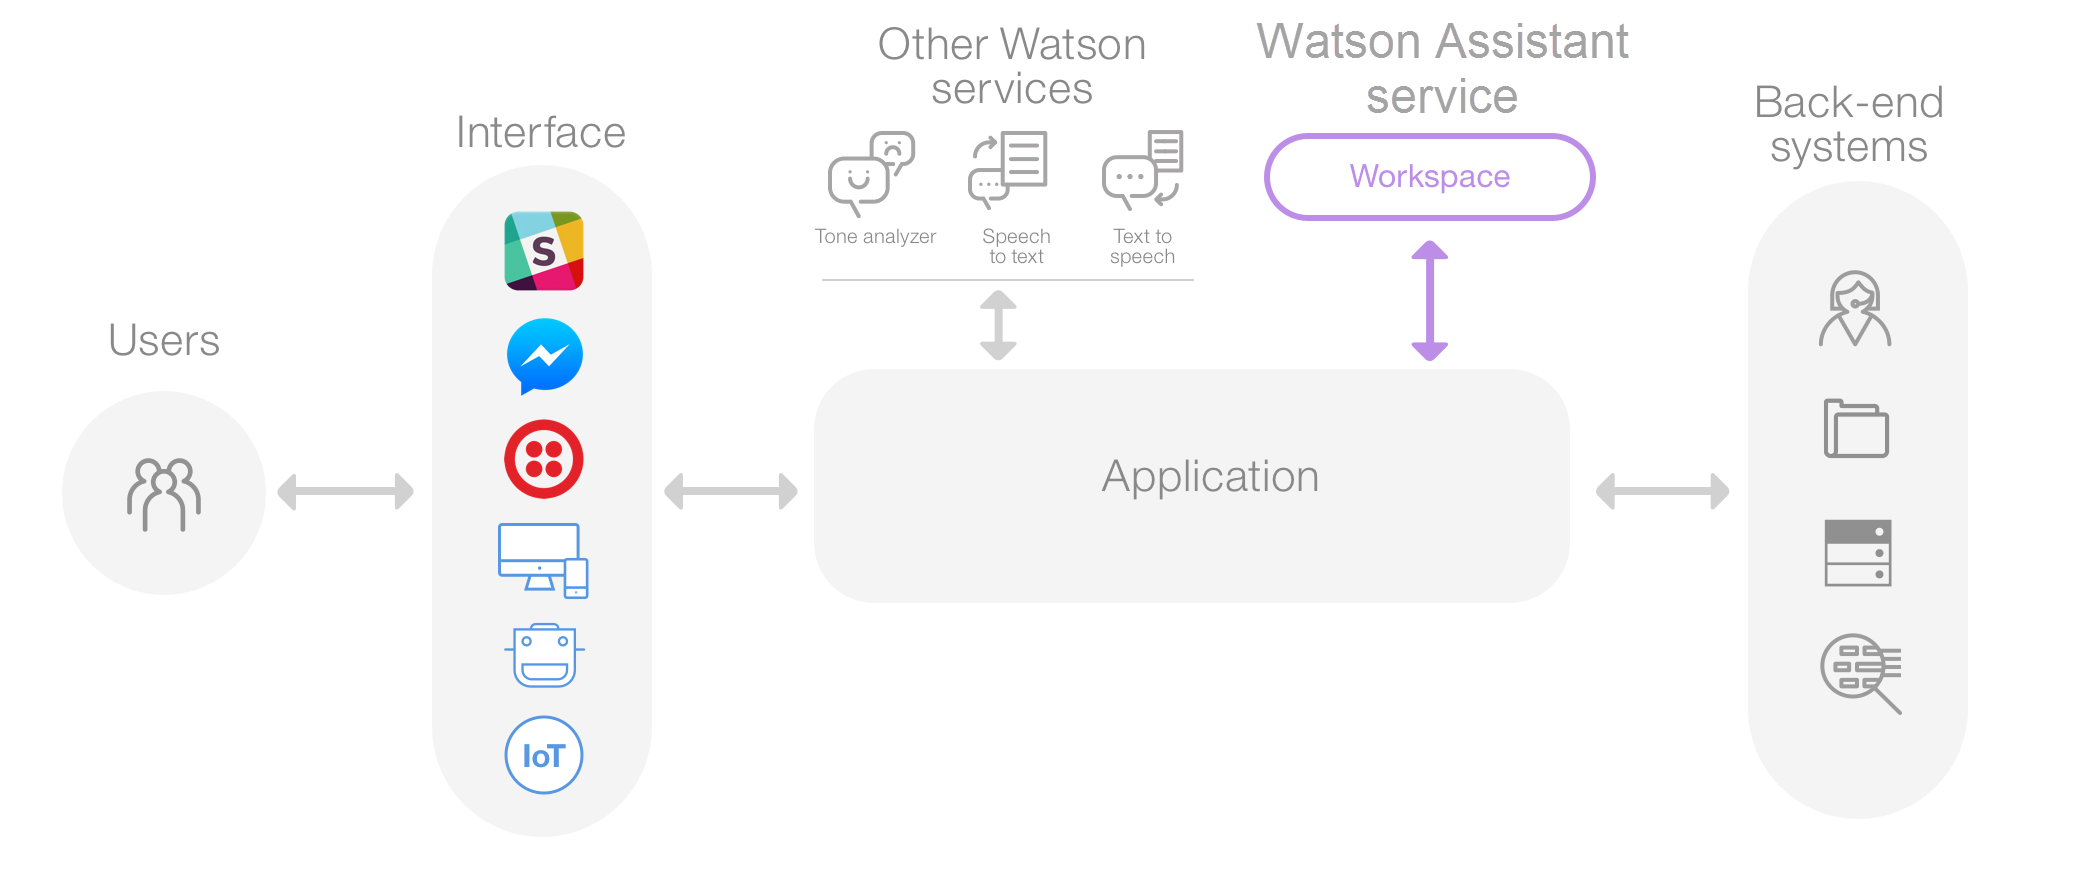
\includegraphics[scale=.2]{images/conversation_arch_overview}
	\label{conversation_arch_overview}
\end{figure}
\begin{itemize}
	\item Build a solution that understands natural-language input and uses machine learning to respond to customers in a way that simulates a conversation between humans.
\end{itemize}
\end{frame}

\begin{frame}
\frametitle{Getting started tutorial (part one)}
\begin{itemize}
	\item 
\end{itemize}
\end{frame}

\begin{frame}
\frametitle{References}
\begin{enumerate}
	\item 
\end{enumerate}
\end{frame}


\end{document}